% Options for packages loaded elsewhere
\PassOptionsToPackage{unicode}{hyperref}
\PassOptionsToPackage{hyphens}{url}
\PassOptionsToPackage{dvipsnames,svgnames,x11names}{xcolor}
%
\documentclass[
  a4paper,
  DIV=11,
  numbers=noendperiod]{scrartcl}

\usepackage{amsmath,amssymb}
\usepackage{lmodern}
\usepackage{iftex}
\ifPDFTeX
  \usepackage[T1]{fontenc}
  \usepackage[utf8]{inputenc}
  \usepackage{textcomp} % provide euro and other symbols
\else % if luatex or xetex
  \usepackage{unicode-math}
  \defaultfontfeatures{Scale=MatchLowercase}
  \defaultfontfeatures[\rmfamily]{Ligatures=TeX,Scale=1}
\fi
% Use upquote if available, for straight quotes in verbatim environments
\IfFileExists{upquote.sty}{\usepackage{upquote}}{}
\IfFileExists{microtype.sty}{% use microtype if available
  \usepackage[]{microtype}
  \UseMicrotypeSet[protrusion]{basicmath} % disable protrusion for tt fonts
}{}
\makeatletter
\@ifundefined{KOMAClassName}{% if non-KOMA class
  \IfFileExists{parskip.sty}{%
    \usepackage{parskip}
  }{% else
    \setlength{\parindent}{0pt}
    \setlength{\parskip}{6pt plus 2pt minus 1pt}}
}{% if KOMA class
  \KOMAoptions{parskip=half}}
\makeatother
\usepackage{xcolor}
\setlength{\emergencystretch}{3em} % prevent overfull lines
\setcounter{secnumdepth}{-\maxdimen} % remove section numbering
% Make \paragraph and \subparagraph free-standing
\ifx\paragraph\undefined\else
  \let\oldparagraph\paragraph
  \renewcommand{\paragraph}[1]{\oldparagraph{#1}\mbox{}}
\fi
\ifx\subparagraph\undefined\else
  \let\oldsubparagraph\subparagraph
  \renewcommand{\subparagraph}[1]{\oldsubparagraph{#1}\mbox{}}
\fi

\usepackage{color}
\usepackage{fancyvrb}
\newcommand{\VerbBar}{|}
\newcommand{\VERB}{\Verb[commandchars=\\\{\}]}
\DefineVerbatimEnvironment{Highlighting}{Verbatim}{commandchars=\\\{\}}
% Add ',fontsize=\small' for more characters per line
\usepackage{framed}
\definecolor{shadecolor}{RGB}{241,243,245}
\newenvironment{Shaded}{\begin{snugshade}}{\end{snugshade}}
\newcommand{\AlertTok}[1]{\textcolor[rgb]{0.68,0.00,0.00}{#1}}
\newcommand{\AnnotationTok}[1]{\textcolor[rgb]{0.37,0.37,0.37}{#1}}
\newcommand{\AttributeTok}[1]{\textcolor[rgb]{0.40,0.45,0.13}{#1}}
\newcommand{\BaseNTok}[1]{\textcolor[rgb]{0.68,0.00,0.00}{#1}}
\newcommand{\BuiltInTok}[1]{\textcolor[rgb]{0.00,0.23,0.31}{#1}}
\newcommand{\CharTok}[1]{\textcolor[rgb]{0.13,0.47,0.30}{#1}}
\newcommand{\CommentTok}[1]{\textcolor[rgb]{0.37,0.37,0.37}{#1}}
\newcommand{\CommentVarTok}[1]{\textcolor[rgb]{0.37,0.37,0.37}{\textit{#1}}}
\newcommand{\ConstantTok}[1]{\textcolor[rgb]{0.56,0.35,0.01}{#1}}
\newcommand{\ControlFlowTok}[1]{\textcolor[rgb]{0.00,0.23,0.31}{#1}}
\newcommand{\DataTypeTok}[1]{\textcolor[rgb]{0.68,0.00,0.00}{#1}}
\newcommand{\DecValTok}[1]{\textcolor[rgb]{0.68,0.00,0.00}{#1}}
\newcommand{\DocumentationTok}[1]{\textcolor[rgb]{0.37,0.37,0.37}{\textit{#1}}}
\newcommand{\ErrorTok}[1]{\textcolor[rgb]{0.68,0.00,0.00}{#1}}
\newcommand{\ExtensionTok}[1]{\textcolor[rgb]{0.00,0.23,0.31}{#1}}
\newcommand{\FloatTok}[1]{\textcolor[rgb]{0.68,0.00,0.00}{#1}}
\newcommand{\FunctionTok}[1]{\textcolor[rgb]{0.28,0.35,0.67}{#1}}
\newcommand{\ImportTok}[1]{\textcolor[rgb]{0.00,0.46,0.62}{#1}}
\newcommand{\InformationTok}[1]{\textcolor[rgb]{0.37,0.37,0.37}{#1}}
\newcommand{\KeywordTok}[1]{\textcolor[rgb]{0.00,0.23,0.31}{#1}}
\newcommand{\NormalTok}[1]{\textcolor[rgb]{0.00,0.23,0.31}{#1}}
\newcommand{\OperatorTok}[1]{\textcolor[rgb]{0.37,0.37,0.37}{#1}}
\newcommand{\OtherTok}[1]{\textcolor[rgb]{0.00,0.23,0.31}{#1}}
\newcommand{\PreprocessorTok}[1]{\textcolor[rgb]{0.68,0.00,0.00}{#1}}
\newcommand{\RegionMarkerTok}[1]{\textcolor[rgb]{0.00,0.23,0.31}{#1}}
\newcommand{\SpecialCharTok}[1]{\textcolor[rgb]{0.37,0.37,0.37}{#1}}
\newcommand{\SpecialStringTok}[1]{\textcolor[rgb]{0.13,0.47,0.30}{#1}}
\newcommand{\StringTok}[1]{\textcolor[rgb]{0.13,0.47,0.30}{#1}}
\newcommand{\VariableTok}[1]{\textcolor[rgb]{0.07,0.07,0.07}{#1}}
\newcommand{\VerbatimStringTok}[1]{\textcolor[rgb]{0.13,0.47,0.30}{#1}}
\newcommand{\WarningTok}[1]{\textcolor[rgb]{0.37,0.37,0.37}{\textit{#1}}}

\providecommand{\tightlist}{%
  \setlength{\itemsep}{0pt}\setlength{\parskip}{0pt}}\usepackage{longtable,booktabs,array}
\usepackage{calc} % for calculating minipage widths
% Correct order of tables after \paragraph or \subparagraph
\usepackage{etoolbox}
\makeatletter
\patchcmd\longtable{\par}{\if@noskipsec\mbox{}\fi\par}{}{}
\makeatother
% Allow footnotes in longtable head/foot
\IfFileExists{footnotehyper.sty}{\usepackage{footnotehyper}}{\usepackage{footnote}}
\makesavenoteenv{longtable}
\usepackage{graphicx}
\makeatletter
\def\maxwidth{\ifdim\Gin@nat@width>\linewidth\linewidth\else\Gin@nat@width\fi}
\def\maxheight{\ifdim\Gin@nat@height>\textheight\textheight\else\Gin@nat@height\fi}
\makeatother
% Scale images if necessary, so that they will not overflow the page
% margins by default, and it is still possible to overwrite the defaults
% using explicit options in \includegraphics[width, height, ...]{}
\setkeys{Gin}{width=\maxwidth,height=\maxheight,keepaspectratio}
% Set default figure placement to htbp
\makeatletter
\def\fps@figure{htbp}
\makeatother

\usepackage{booktabs}
\usepackage{longtable}
\usepackage{array}
\usepackage{multirow}
\usepackage{wrapfig}
\usepackage{float}
\usepackage{colortbl}
\usepackage{pdflscape}
\usepackage{tabu}
\usepackage{threeparttable}
\usepackage{threeparttablex}
\usepackage[normalem]{ulem}
\usepackage{makecell}
\usepackage{xcolor}
\KOMAoption{captions}{tableheading}
\makeatletter
\makeatother
\makeatletter
\makeatother
\makeatletter
\@ifpackageloaded{caption}{}{\usepackage{caption}}
\AtBeginDocument{%
\ifdefined\contentsname
  \renewcommand*\contentsname{Table of contents}
\else
  \newcommand\contentsname{Table of contents}
\fi
\ifdefined\listfigurename
  \renewcommand*\listfigurename{List of Figures}
\else
  \newcommand\listfigurename{List of Figures}
\fi
\ifdefined\listtablename
  \renewcommand*\listtablename{List of Tables}
\else
  \newcommand\listtablename{List of Tables}
\fi
\ifdefined\figurename
  \renewcommand*\figurename{Figure}
\else
  \newcommand\figurename{Figure}
\fi
\ifdefined\tablename
  \renewcommand*\tablename{Table}
\else
  \newcommand\tablename{Table}
\fi
}
\@ifpackageloaded{float}{}{\usepackage{float}}
\floatstyle{ruled}
\@ifundefined{c@chapter}{\newfloat{codelisting}{h}{lop}}{\newfloat{codelisting}{h}{lop}[chapter]}
\floatname{codelisting}{Listing}
\newcommand*\listoflistings{\listof{codelisting}{List of Listings}}
\makeatother
\makeatletter
\@ifpackageloaded{caption}{}{\usepackage{caption}}
\@ifpackageloaded{subcaption}{}{\usepackage{subcaption}}
\makeatother
\makeatletter
\@ifpackageloaded{tcolorbox}{}{\usepackage[many]{tcolorbox}}
\makeatother
\makeatletter
\@ifundefined{shadecolor}{\definecolor{shadecolor}{rgb}{.97, .97, .97}}
\makeatother
\makeatletter
\makeatother
\ifLuaTeX
  \usepackage{selnolig}  % disable illegal ligatures
\fi
\IfFileExists{bookmark.sty}{\usepackage{bookmark}}{\usepackage{hyperref}}
\IfFileExists{xurl.sty}{\usepackage{xurl}}{} % add URL line breaks if available
\urlstyle{same} % disable monospaced font for URLs
\hypersetup{
  pdftitle={Eurostat EDA},
  pdfauthor={Sindre H. Øveraas, Alen Colakovic \& Sebastian M. Fløysand},
  colorlinks=true,
  linkcolor={blue},
  filecolor={Maroon},
  citecolor={Blue},
  urlcolor={Blue},
  pdfcreator={LaTeX via pandoc}}

\title{Eurostat EDA}
\author{Sindre H. Øveraas, Alen Colakovic \& Sebastian M. Fløysand}
\date{}

\begin{document}
\maketitle
\ifdefined\Shaded\renewenvironment{Shaded}{\begin{tcolorbox}[enhanced, frame hidden, interior hidden, boxrule=0pt, borderline west={3pt}{0pt}{shadecolor}, sharp corners, breakable]}{\end{tcolorbox}}\fi

\hypertarget{eurostat-eda}{%
\subsection{Eurostat EDA}\label{eurostat-eda}}

\hypertarget{meta-data-description}{%
\paragraph{Meta-data description}\label{meta-data-description}}

\hypertarget{nama-10r}{%
\paragraph{Nama 10r}\label{nama-10r}}

Regional accounts are based on the same definitions and concepts as
national accounts, this is because they are a specification of the
national accounts.

\emph{Gross domestic product (GDP) is the standard measure of the value
added created through the production of goods and services in a country
during a certain period. As such, it also measures the income earned
from that production, or the total amount spent on final goods and
services (less imports). While GDP is the single most important
indicator to capture economic activity, it falls short of providing a
suitable measure of people's material well-being for which alternative
indicators may be more appropriate.\\
}@GDPSpendingGross

Our goal with this task is to compare the GDP´s of the different regions
within nations. We will dig deeper into the evelution of the GDP to each
of our given nations aswell as some of their most intriguing regions.

\hypertarget{sub-national-gdp}{%
\subsubsection{Sub-national GDP}\label{sub-national-gdp}}

Country codes: BE - Belgium, BG - Bulgaria, HR - Croatia, IT - Italy, AT
- Austria, SE - Sweden, RS - Serbia

These are the RStudio packages we install and load to do our
calculations.

\begin{Shaded}
\begin{Highlighting}[]
\FunctionTok{library}\NormalTok{(tidyverse)}
\FunctionTok{library}\NormalTok{(vtable)}
\FunctionTok{library}\NormalTok{(dineq)}
\FunctionTok{library}\NormalTok{(dplyr)}
\end{Highlighting}
\end{Shaded}

We downloaded from Eurostat our subset of countries sub-regional GDP
(nama\_10r\_3gdp\_\_custom\_3564935\_linear.csv) and population
(demo\_r\_pjanaggr3\_\_custom\_3579517\_linear.csv) for the years 2000 -
2020. We then calculated the GDP per capita, and named the new data set
``GDP\_Per\_Capita''.

\begin{Shaded}
\begin{Highlighting}[]
\FunctionTok{library}\NormalTok{(readr)}
\NormalTok{GDP }\OtherTok{\textless{}{-}} \FunctionTok{read.csv}\NormalTok{(}\StringTok{\textquotesingle{}nama\_10r\_3gdp\_\_custom\_3564935\_linear.csv\textquotesingle{}}\NormalTok{)}
\NormalTok{Population }\OtherTok{\textless{}{-}} \FunctionTok{read\_csv}\NormalTok{(}\StringTok{"demo\_r\_pjanaggr3\_\_custom\_3579517\_linear.csv"}\NormalTok{)}

\NormalTok{gdpdata }\OtherTok{\textless{}{-}}\NormalTok{ GDP }\SpecialCharTok{\%\textgreater{}\%}
  \FunctionTok{rename}\NormalTok{(}\AttributeTok{Year =}\NormalTok{ TIME\_PERIOD, }\AttributeTok{GDP =}\NormalTok{ OBS\_VALUE, }\AttributeTok{Region =}\NormalTok{ geo)}

\NormalTok{populationdata }\OtherTok{\textless{}{-}}\NormalTok{ Population }\SpecialCharTok{\%\textgreater{}\%}
  \FunctionTok{rename}\NormalTok{(}\AttributeTok{Year =}\NormalTok{ TIME\_PERIOD, }\AttributeTok{Population =}\NormalTok{ OBS\_VALUE, }\AttributeTok{Region =}\NormalTok{ geo)}

\NormalTok{GDP\_Per\_Capita }\OtherTok{\textless{}{-}}\NormalTok{ gdpdata }\SpecialCharTok{\%\textgreater{}\%}
  \FunctionTok{left\_join}\NormalTok{(populationdata, }\AttributeTok{by=}\FunctionTok{c}\NormalTok{(}\StringTok{"Region"}\NormalTok{, }\StringTok{"Year"}\NormalTok{)) }\SpecialCharTok{\%\textgreater{}\%}
  \FunctionTok{select}\NormalTok{(Region, Year, GDP, Population) }\SpecialCharTok{\%\textgreater{}\%}
  \FunctionTok{mutate}\NormalTok{(}
    \AttributeTok{GDP\_capita =}\NormalTok{ (GDP }\SpecialCharTok{*} \DecValTok{1000000}\NormalTok{)}\SpecialCharTok{/}\NormalTok{Population)}
\end{Highlighting}
\end{Shaded}

To report our descriptive statistics on GDP per capita, we used the
summary command. This gave us the following descriptive statistics on
the variables GDP, population and GDP capita.

\begin{verbatim}
      GDP              Population        GDP_capita   
 Min.   :    74.55   Min.   :  20320   Min.   : 1087  
 1st Qu.:  1738.28   1st Qu.: 164518   1st Qu.:17180  
 Median :  5614.05   Median : 273920   Median :25185  
 Mean   : 10238.24   Mean   : 406217   Mean   :24191  
 3rd Qu.: 10640.23   3rd Qu.: 429030   3rd Qu.:31351  
 Max.   :181212.88   Max.   :4355725   Max.   :72062  
                     NA's   :771       NA's   :771    
\end{verbatim}

To calculate the population watertight GDP Ginie coefficient, we used
the following command.

\begin{Shaded}
\begin{Highlighting}[]
\FunctionTok{gini.wtd}\NormalTok{(GDP\_Per\_Capita}\SpecialCharTok{$}\NormalTok{GDP\_capita, }\AttributeTok{weights =}\NormalTok{ GDP\_Per\_Capita}\SpecialCharTok{$}\NormalTok{Population)}
\end{Highlighting}
\end{Shaded}

\begin{verbatim}
[1] 0.2603924
\end{verbatim}

To calculate the population watertight GDP Ginie coefficents for the
European NUTS2 level, we used the following commands.

\begin{Shaded}
\begin{Highlighting}[]
\NormalTok{GDP\_Per\_Capita }\OtherTok{\textless{}{-}}\NormalTok{ GDP\_Per\_Capita }\SpecialCharTok{\%\textgreater{}\%}  
  \FunctionTok{mutate}\NormalTok{(}\AttributeTok{NUTS2 =} \FunctionTok{substr}\NormalTok{(GDP\_Per\_Capita}\SpecialCharTok{$}\NormalTok{Region,}\DecValTok{1}\NormalTok{,}\DecValTok{4}\NormalTok{))}

\NormalTok{GDP\_Per\_Capita }\OtherTok{\textless{}{-}}\NormalTok{ GDP\_Per\_Capita }\SpecialCharTok{\%\textgreater{}\%}  
  \FunctionTok{mutate}\NormalTok{(}\AttributeTok{NUTS =} \FunctionTok{substr}\NormalTok{(GDP\_Per\_Capita}\SpecialCharTok{$}\NormalTok{Region,}\DecValTok{1}\NormalTok{,}\DecValTok{2}\NormalTok{))}

\NormalTok{GDP\_Per\_Capita  }\SpecialCharTok{\%\textless{}\textgreater{}\%}
  \FunctionTok{group\_by}\NormalTok{(NUTS2) }\SpecialCharTok{\%\textgreater{}\%}
  \FunctionTok{na.exclude}\NormalTok{(GDP\_Per\_Capita) }\SpecialCharTok{\%\textgreater{}\%}
  \FunctionTok{mutate}\NormalTok{(}\AttributeTok{GINI\_NUTS2 =} \FunctionTok{gini.wtd}\NormalTok{(GDP\_capita, }\AttributeTok{weights =}\NormalTok{ Population)) }\SpecialCharTok{\%\textgreater{}\%}
  \FunctionTok{ungroup}\NormalTok{()}
\end{Highlighting}
\end{Shaded}

To summarize the data of the Ginie coefficients, we once more used the
summarize command. We see here the gap between minimum and maximum is
more then 10 times difference from 0.03367 to 0.36569 but the mean and
median is at 0.09839 and 0.11800 which implies that the majority is
located in closer to the minium and middle.

\begin{verbatim}
   GINI_NUTS2     
 Min.   :0.03367  
 1st Qu.:0.07065  
 Median :0.09839  
 Mean   :0.11800  
 3rd Qu.:0.15525  
 Max.   :0.36569  
\end{verbatim}

For visualization of our data (the Ginie coefficients for the European
NUTS2 level of our selected countries), we produced a density plot and
histogram, by the use of the ggplot2 package.

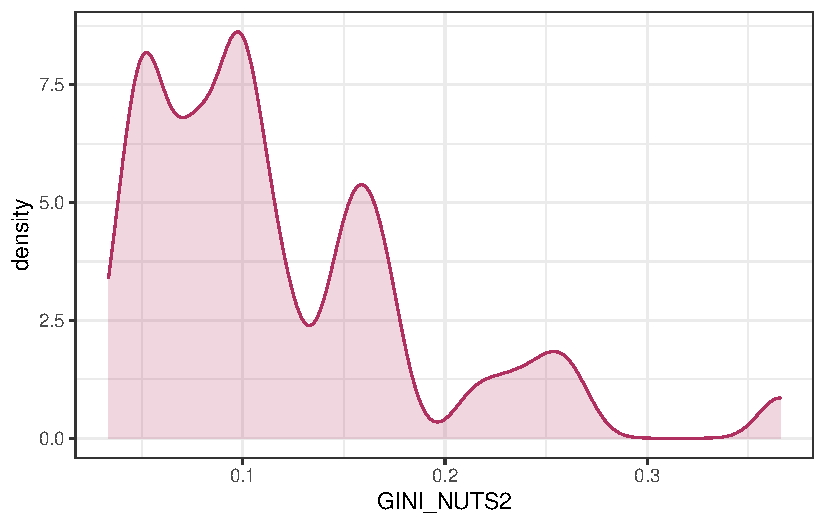
\includegraphics{Eurostat-EDA_files/figure-pdf/unnamed-chunk-8-1.pdf}

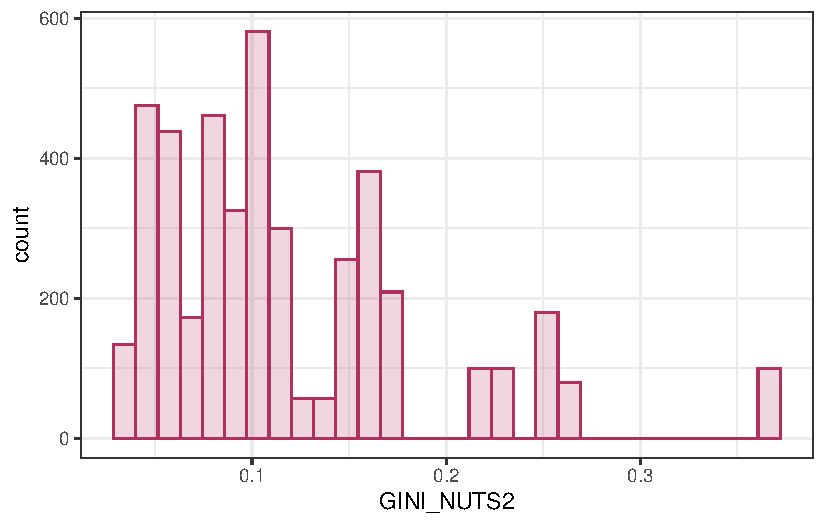
\includegraphics{Eurostat-EDA_files/figure-pdf/unnamed-chunk-9-1.pdf}

Looking at the plot above there is one outlier up against 0.4 with
around 100 observations. The same result also seem to occur in the
density plot. The majority is seen around 0.1 with a descending decline.

-\/-\/-\/-\/-\/-\/-\/-\/-\/-

\textbf{We made a variety of diagrams to show the difference between
some countries and regions.}

For this diagram we picked and divided the countries in to their
respected sub-regions and catagorized them, before comparing.\\

Central and Eastern Europe: Croatia, Serbia and Bulgaria\\

South Europe: Italy\\

Northern Europe: Sweden\\

Western Europe: Austria and Belgium\\

(Catagorized collected from wikipedia :
(\textbf{FileEuropeanSubregions?}) )

With this diagram, we can see the GDP of the different areas and their
rise and fall from the 2000 to 2020.

\textbf{**explain what we see}**\\

\begin{center}\rule{0.5\linewidth}{0.5pt}\end{center}

Further on we wish to highlight some of the regions within countries to
see differences in GDP. There are some countries with wider gaps between
them, and makes this a insightful visual representation. We dig deeper
into Sweden where we used the regions: Stockholm, Uppsala and Gotland.
With these we se some big gaps when it comes to GDP and how Stockholm
alone raises the country´s collective GDP. In the diagram below we also
show the GDP Per Capita in each region.*** The simple reason behind the
difference is the location of Stockholm and that it is the capital of
sweden, as well as being one of the major industrial cities in Sweden
also called industrial cluster area.

***Do more calulations on differences on regional levels and give
further explanations***\\

\hfill\break

**** show 2 diagrams of gdp aswell as gdp per capita ****



\end{document}
